%
% problemstellung.tex -- Beispiel-File für die Beschreibung des Problems
%
% (c) 2020 Prof Dr Andreas Müller, Hochschule Rapperswil
%
\section{Problemstellung
\label{taylor:section:problemstellung}}
Um die nummerische Approximation an einem konkreten Beispiel zeigen zu können wird hier die Logistische Funktion \ref{taylor:section:logistifunction} analysiert.
Es handelt sich hierbei um eine begrenze Wachstumsfunktion. 
Mit dieser Funktion kann zum Beispiel der Verlauf einer Krankheit abgebildet werden, der Lebenszyklus eines Produktes oder auch Zerfallsprozesse beschrieben werden.

L = Endwert, k = Wachstumsrate
\begin{equation}
	y'
	=
	k\cdot y(L-y)
	\label{taylor:section:logistifunction}
\end{equation}

Da wir nur eine Unbekante benötigen normieren wir den Endwert L auf 1.
Der Endwert entspricht zum Beispiel der Anzahl Infiszierten am Ender einer Krankheitsepidemie.
In der Abbildung ~\ref{taylor:section:fig:DGLDarstellung} ist zu erkennen, dass der Wachstumsfaktor k bestimmt wie steil die Funktion wird.
Somit haben wir nun ein Feld gegeben, indem wir in jedem möglichen Punkt der Funktion eine genau definierte Steigung, bzw. ein genau definiertes k haben.
Um aber das k und damit die DGL bestimmen zu können müssten wir diese mühsam ausrechnen.
Deshalb macht es in einem solchen Fall Sinn die Funktion mit kleinen Schritten zu erarbeiten und somit das mathematisch komplizierte Lösungsverfahren zu umgehen.

\begin{figure}[h]
	\centering
	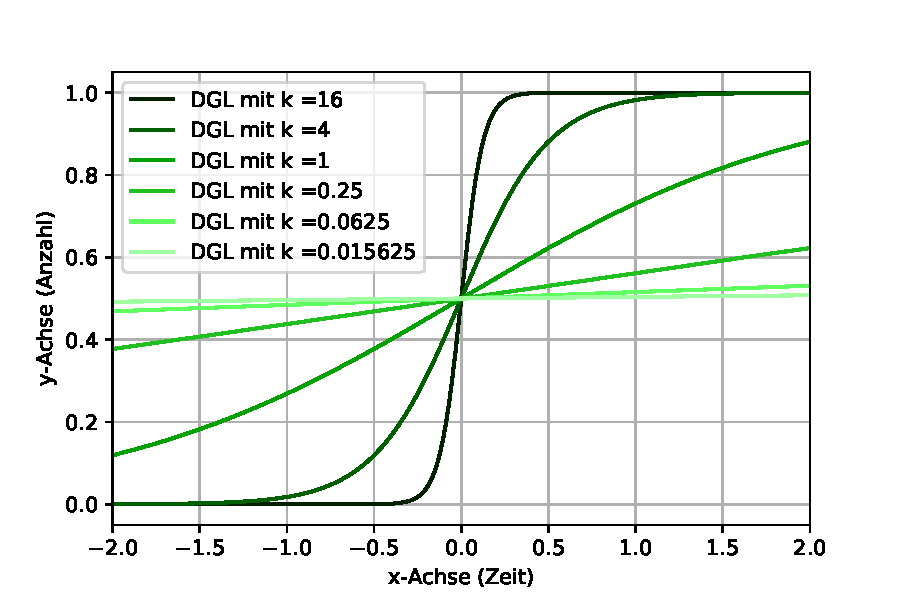
\includegraphics[width=12cm]{papers/taylor/taylorPictures/DGLDarstellung.pdf}
	\caption{Logistische Funktion in Abhängigkeit von k}
	\label{taylor:section:fig:DGLDarstellung}
\end{figure}

Da wir für die Taylor Approximation die Ableitungen bis zur n-ten Ordnung benötigen müssen diese natürlich bekannt sein.

\begin{equation}
	y'=k\cdot (y-y^{2})
\end{equation}

\begin{equation}
	y''=k\cdot (y'-2y'\cdot y)
\end{equation}

\begin{equation}
	y'''=k\cdot (y''-2y''\cdot y+y'^{2})
\end{equation}

\begin{equation}
	y''''=k\cdot (y'''-2y'''\cdot y+3y''\cdot y')
\end{equation}

\begin{equation}
	y'''''=k\cdot (y''''-2y'''\cdot y+4y''\cdot y'+3y''^{2})
\end{equation}

\begin{equation}
	k=\frac{-\ln{(\frac{1}{y}-1)}}{x}
\end{equation}

\section{Vorgehen}
\label{taylor:subsection:Vorgehen}
Ähnlich wie beim Runge-Kutta Verfahren soll mit kleinen Schritten der Verlauf der Funktion ausgehend von einen Anfangswert ermittelt werden.
Die Taylor-Reihe setzt sich zusammen aus der korrekten Gewichtung der Ableitungen bis zur gewünschten Ordnung.
Je höher der Grad, desto grösser ist der Bereich um den Punkt der Auswertung herum in dem die Taylor Approximation mit der tatsächlichen Funktion übereinstimmt.
Die Taylorfunktion am Auswertungspunkt wird nun als Approximation der DGL genommen um zum nächsten Punkt zu gelangen.
Dort werden erneut die Ableitungen ausgerechnet und eine weitere Approximationsfunktion aufgestellt, mit der dann der darauf folgende Punkt bestimmen wird.
Je kleiner nun die Schrittweite gewählt wird, desto weniger spielen höhere Ableitungen, beziehungsweise höhere Frequenzanteile, eine Rolle.
In der Abbildung~\ref{taylor:section:fig:LogisticFunctionApproximation} sieht man ein Vergleich des Runge-Kutta Verfahrens und des Taylor Verfahrens.

\begin{figure}[h]
	\begin{center}
	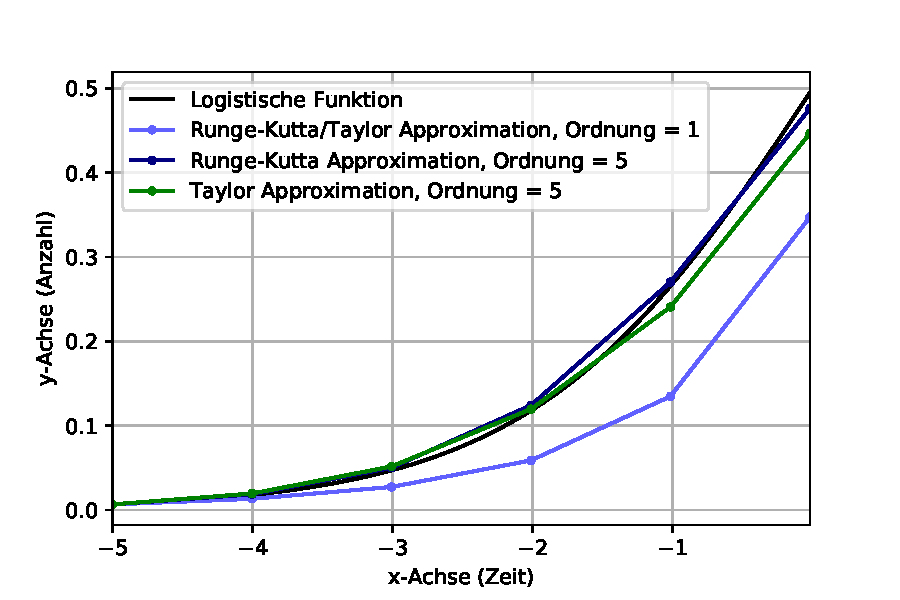
\includegraphics[width=12cm]{papers/taylor/taylorPictures/LogisticFunction.pdf}
	\caption{Gleichung und Approximationen der Logistische Funktion für k=1, Approximationen mit 5 Schritten von -5 bis -0.02 und Startwert der selbe wie bei k=1}
	\label{taylor:section:fig:LogisticFunctionApproximation}
	\end{center}
\end{figure}

\begin{equation}
	f_{T}(x,a)
	=
	\sum_{n=0}^{\infty}{\frac{f^{(n)}\cdot a}{n!}}\cdot (x-a)^{n}
	\label{taylor:section:taylor}
\end{equation}
$f_{T}(x,a)$ = Taylor Funktion


\begin{tabular}[h]{|l|l|l|l|l|l|}
	\hline
	Runge-Kutta & k = 1 & k = 2 & k = 3 & k = 4 & k = 5\\
	\hline
	n = 1 & 0.45519 & 0.31990 & 0.11077 & 4.68470e-2 & 6.19930e-2\\
	\hline
	n = 2 & 0.38755 & 3.85299e-2 & 5.97521e-2 & 1.05400e-2 & 4.07133e-2\\
	\hline
	n = 5 & 0.14751 & 2.39004e-2 & 2.59349e-2 & 1.33486e-2 & 1.88327e-2\\
	\hline
	n = 10 & 6.88690e-2 & 4.37589e-3 & 4.37432e-3 & 2.58736e-3 & 3.50711e-3\\
	\hline
	n = 1000 & 6.19312e-4 & 5.23506e-7 & 1.84704e-07 & 1.85763e-7 & 1.85765e-07\\
	\hline
	n = 100000 & 6.18453e-6 & 5.13468e-11 & 1.96497e-11 & 1.96507e-11 & 1.96507e-11\\
	\hline
\end{tabular}

k = Ordnung, n = Schritte, Start = -5, Ende = -0.02, (letzte Ziffer abgerundet)

\begin{tabular}[h]{|l|l|l|l|l|l|}
	\hline
	Taylor & k = 1 & k = 2 & k = 3 & k = 4 & k = 5\\
	\hline
	n = 1 & 0.45519 & 0.27840 & 0.27948 & 0.29078 & 0.29515\\
	\hline
	n = 2 & 0.38755 & 0.20040 & 0.19400 & 0.19579 & 0.19663\\
	\hline
	n = 5 & 0.14751 & 5.30816e-2 & 4.80256e-2 & 4.79241e-2 & 4.79851e-2\\
	\hline
	n = 10 & 6.88690e-2 & 1.60657e-2 & 1.38830e-2 & 1.38673e-2 & 1.38751e-2\\
	\hline
	n = 1000 & 6.19312e-4 & 2.11126e-6 & 1.90164e-6 & 1.90183e-6 & 1.90183e-6\\
	\hline
	n = 100000 & 6.18453e-6 & 2.10965e-10 & 1.90226e-10 & 1.90226e-10 & 1.90226e-10\\
	\hline
\end{tabular}

k = Ordnung, n = Schritte, Start = -5, Ende = -0.02, (letzte Ziffer abgerundet)

\begin{figure}[h]
	\centering
	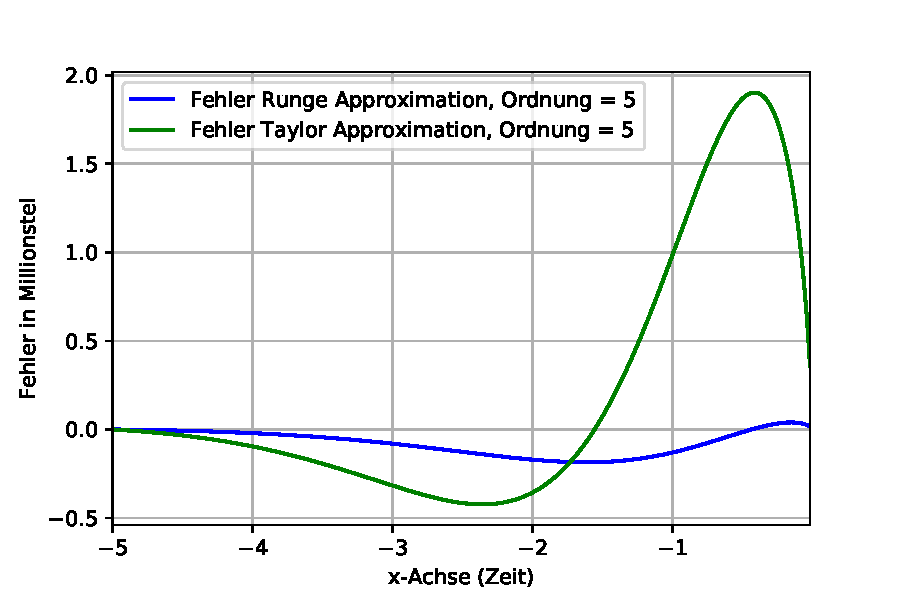
\includegraphics[width=12cm]{papers/taylor/taylorPictures/FehlerRungeUndTaylor.pdf}
	\caption{Fehler der Approximationen bei 1000 Schritten von -5 bis -0.02 und Startwert der selbe wie bei k=1}
	\label{taylor:section:fig:FehlerRungeTaylor}
\end{figure}

\subsection{Auswertung des Vergleiches}
\label{taylor:subsection:Auswertung}
Die ersten Spalten der beiden Verfahren sehen gleich aus, weil die Approximationen erster Ordnung auf das selbe herauskommen.
Nämlich auf das Approximieren der Funktion mit geraden erster Ordnung, was der Steigung im Auswertungspunkt entspricht.

Beim Punkt n=1 und k=2 ist die Taylor Approximation besser als Runge-Kutta.
Eine Approximation mit dem Grad 2 und einem Schritt über eine sich so stark verändernde Kurve ist aber eher ein Glückstreffer als ein mathematischer Erfolg.
Im Allgemeinen kann gesagt werden dass das Runge-Kutta Verfahren in diesem Fall ein kleineren Fehler aufweist. Dies ist auch in der Abbildung \ref{taylor:section:fig:FehlerRungeTaylor} zu sehen.

\section{Probleme mit der Logistischen Funktion}
\label{taylor:subsection:Probleme}
Die Logistische Funktion wurde gewählt weil es eine anschauliche, nichtlineare Differentialgleichung ist welche sich somit gut eignet um das Runge-Kutta Verfahren mit dem Taylor Verfahren zu vergleichen.
Dabei traten allerdings folgende 2 Probleme auf.

\subsection{Konvergenz}
\label{taylor:subsection:Konvergenz}
Wie in Abbildung 
\ref{taylor:section:fig:DGLDarstellung}
ersichtlich ist, konvergiert die DGL im Punkt 0 auf 0.5 und bei $\infty$ auf 1.
Wird nun also diese DGL approximiert, dann ist sowieso klar auf welchem Wert wir ungefähr landen werden.
Um eine Aussagekräftige Antwort auf die Frage der Qualität geben zu können wurden die Fehler über den ganzen Verlauf der Approximation verglichen. Siehe dazu Abbildung \ref{taylor:section:fig:FehlerRungeTaylor}.

\subsection{Nicht erlaubter 0-Punkt}
\label{taylor:subsection:0Punkt}
Wie in Abbildung 
\ref{taylor:section:fig:DGLDarstellung}
klar dargestellt ist, ist die Ableitung in direkter Umgebung vom Punkt (0, 0.5) zwischen 0 und $\infty$.
Wenn also eine Approximation der DGL sich durch diesen Punkt erarbeiten möchte, wird sie durch einen auch noch so kleinen Fehler eine ganz andere Ableitung berechnen und somit völlig anders verlaufen.
Um dies zu umgehen wurde einfach nicht durch diesen Wendepunkt gegangen, sondern nur bis 0.02 davor.
Man könnte nun aber die erhaltenen linke Kurve an dem Wendepunkt punktspiegeln und hätte so die zweite Hälfte ebenfalls, welche somit sowieso redundant und für uns nicht intressant ist.

%\nameref
%\pageref{}
%\numref
%\ref{taylor:section:loesung}.
%\ref{taylor:section:folgerung}.


